\begin{figure}[t]
\begin{centering}
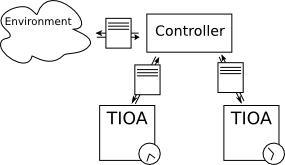
\includegraphics[scale=0.8]{images/ecdar_architecture_2.png}
\par\end{centering}

\caption{Schematic of the architecture of our ECDAR implementation.}
\end{figure}

The architecture we chose is based upon the work of Amnell et
al.\cite{amnell_code_2002} with some modifications. Communication between
automata is implemented as message passing between a controller and automata,
where automata send messages to the controller by traversing over output
edges. This is different in actual ECDAR, where automata communicate through
message passing directly between each other. However, by choosing a slightly
different architecture, we can unify the message system in the implementation,
handling all messages central and also not distinguishing between a message
coming from the environment or a message send by an automaton. The resulting
behavior is equal.

Automata need to execute in quasi-parallel. In the implementation they are run
in a classical threading architecture that does not require multiple processor
units. Since there is no communication between automata directly, we can
minimize synchronizing between threads (see more on synchronizing in
Sec. \ref{subsec:synch}).

The following overview will give further implementation details on each
component of ECDAR as we implemented it. Each component is illustrated with a
short code example, implementing ECDAR's ``University''
example\footnote{\url{http://people.cs.aau.dk/adavid/ecdar/examples.html#university}}. For
clarity, we omit the framework implementation and focus on the generated code.

\subsubsection{Controller.}

\begin{figure}[t]
\lstinputlisting[linerange={6-11,63-63}]{../dk.itu.ecdar.text.generator.mockup/src/dk/itu/ecdar/text/generator/mockup/university/UniversityController.java}
\caption{Example of controller code.}
\label{controller-example}
\end{figure}

The controller holds all automata given in the specification and notifies them
about received messages. It is a singleton, accessible in a static fashion.
This property is useful for sending messages to the controller.

\subsubsection{TIOA.}

The implementation of timed I/O automata holds a set of locations and a
reference to the location it is currently at. The TIOA is executed by a thread
that keeps checking for available edges and traverses along these as soon as
they become enabled. To check if an edge is available, let $E_{s\rightarrow t}$
be an edge where $s,\, t$ are start and target locations
respectively. Furthermore, let $g(E)$ be a function evaluating the guard of an
edge $E$ and $I(l)$ a function evaluating the invariant of a location $l$. Our
implementation uses $g'(E_{s\rightarrow t})=g(E_{s\rightarrow t})\wedge I(t)$ to
check if $E_{s\rightarrow t}$ is available. We do not check the invariant of the
source location because if the source location's invariant was violated, the
system would already be in a deadlock. This cannot be true, as we assume that
the system is verified.

\begin{figure}[t]
\lstinputlisting[linerange={8-8,157-170}]{../dk.itu.ecdar.text.generator.mockup/src/dk/itu/ecdar/text/generator/mockup/university/Machine.java}
\caption{Example of TIOA code.}
\label{tioa-example}
\end{figure}

Additionally, the automaton has the ability to return the current
local clock state (see \ref{implementation-presumptions}) and to
reset the clock. We use the same notion of clocks as \cite{amnell_code_2002},
where time on the local clock is the difference between the current
time on the system clock and the time the local clock was started.
Resetting the local clock means to use the current system clock time
as the new start time (see Fig. \ref{tioa-example}).

\subsubsection{Locations.}

\begin{figure}[t]
\lstinputlisting[linerange={98-119}]{../dk.itu.ecdar.text.generator.mockup/src/dk/itu/ecdar/text/generator/mockup/university/Machine.java}
\caption{Example of location code.}
\label{location-example}
\end{figure}

Each location is associated with a task (see Sec. \ref{subsec:tasks}). Task
execution is implemented in a separate thread so that the execution of the
automaton is never blocked. Locations are implemented as objects holding an
array of edges that point away from it. (See Fig. \ref{location-example})


\subsubsection{Edges.}
\label{subsubsec:edges}

\begin{figure}[t]
\lstinputlisting[linerange={11-24}]{../dk.itu.ecdar.text.generator.mockup/src/dk/itu/ecdar/text/generator/mockup/university/Machine.java}
\caption{Example of edge code.}
\label{edge-example}
\end{figure}

An edge holds a reference to the location which the parent automaton
will be at after traversing this very edge. Edges can be asked if
they will be available at a given time. This is implemented to enable
lazy waiting in the automaton's traversal checker. Each edge is associated
with some input. If an edge is controllable, it will be triggered
if the automaton is notified at this input. If it is uncontrollable,
it will send its input to the controller. Furthermore, edges have
access to the clock of the parent automaton to reset it appropriately.

The implementation makes a class-wise distinction between input edges
(i.e. edges that are traversed when a corresponding message was received) and
output edges (edges that send messages on traversal) and hard-codes the behavior
in the framework, e.g. messaging the controller (see Fig. \ref{edge-example}).
